\subsection{Setzeinheit}
Die Wahl der Spindel und des Spindelantriebes haben einen entscheidenden Einfluss auf die Erfüllung des Setzprozesses innerhalb der vorgegeben Zeit. Parameter wie Steigung, Spindeldurchmesser und Material der Spindel wirken sich direkt auf die Massenträgheit und somit auf das erforderliche Beschleunigungsmoment aus.

\subsubsection{Auslegung Spindeltrieb}
Die Subkapitel befasst sich mit der Auslegung und Berechnung des Spindeltriebes. Dabei sind Berechnungen in zusammengefasster Form dargestellt. Der vollständige Rechenweg und die detailierte Vorgehensweise sind im Anhang (\textbf{Datei XY}) zu entnehmen.

Gegeben durch den Setzprozess und die Geometrie sind folgende Daten:
	\begin{figure}[H]
	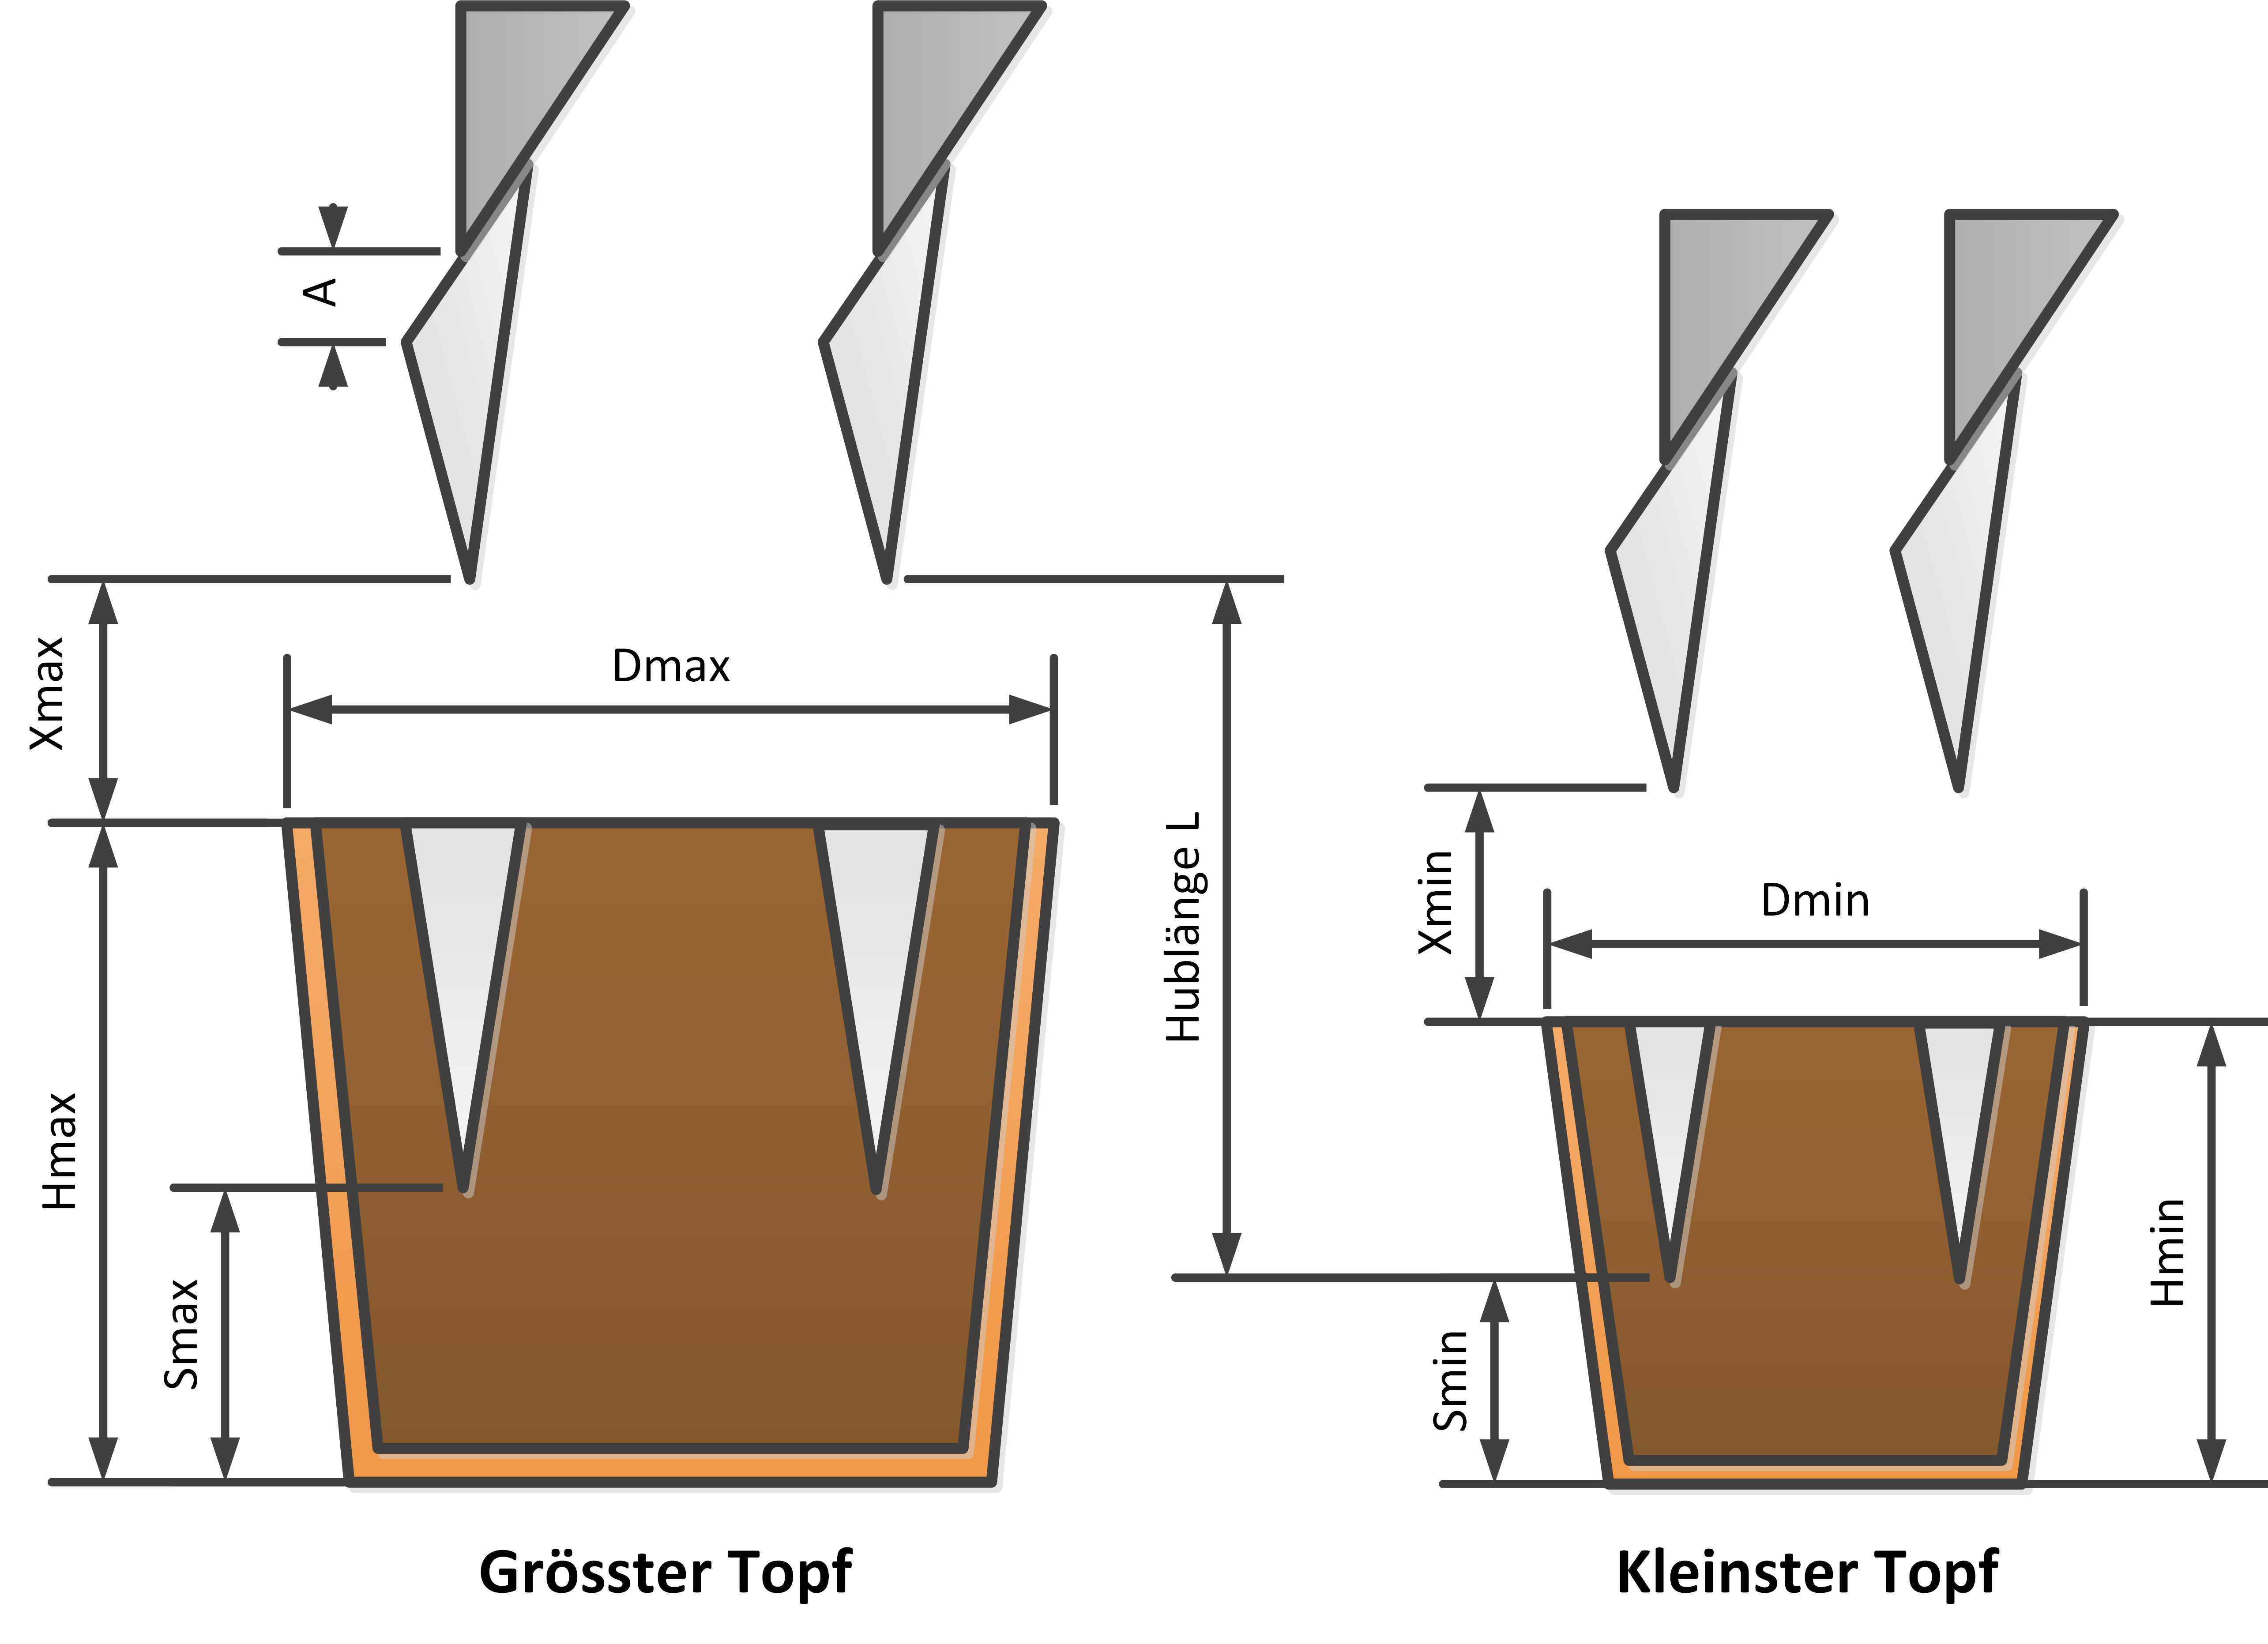
\includegraphics[width=1\textwidth]{Illustrationen/6-Umsetzung/topfgeometrie.png}
	\caption{Geometrie der Töpfe und des Setzprozess}
	\label{fig:topfgeometrie}
	\end{figure}
Anhand dieser Randbedingungen und den getroffenen Annahmen ergibt sich eine Beschleunigungs- und Bremszeit tb=0.1125s. Bei einem maximalen Hubweg Umax = 72.4mm beträgt die grösste durschnittliche Geschwindigkeit vavmax:

\begin{equation}
v_{avmax}=\frac{U_{max}}{t_{b}}=\frac{72.4mm}{0.1125s}=643.5mm/s
\end{equation}
\newline
Die Geschwindigkeit des Dornes kann streng idealisiert gemäss Abbildung XY dargestellt werden:
	\begin{figure}[H]
	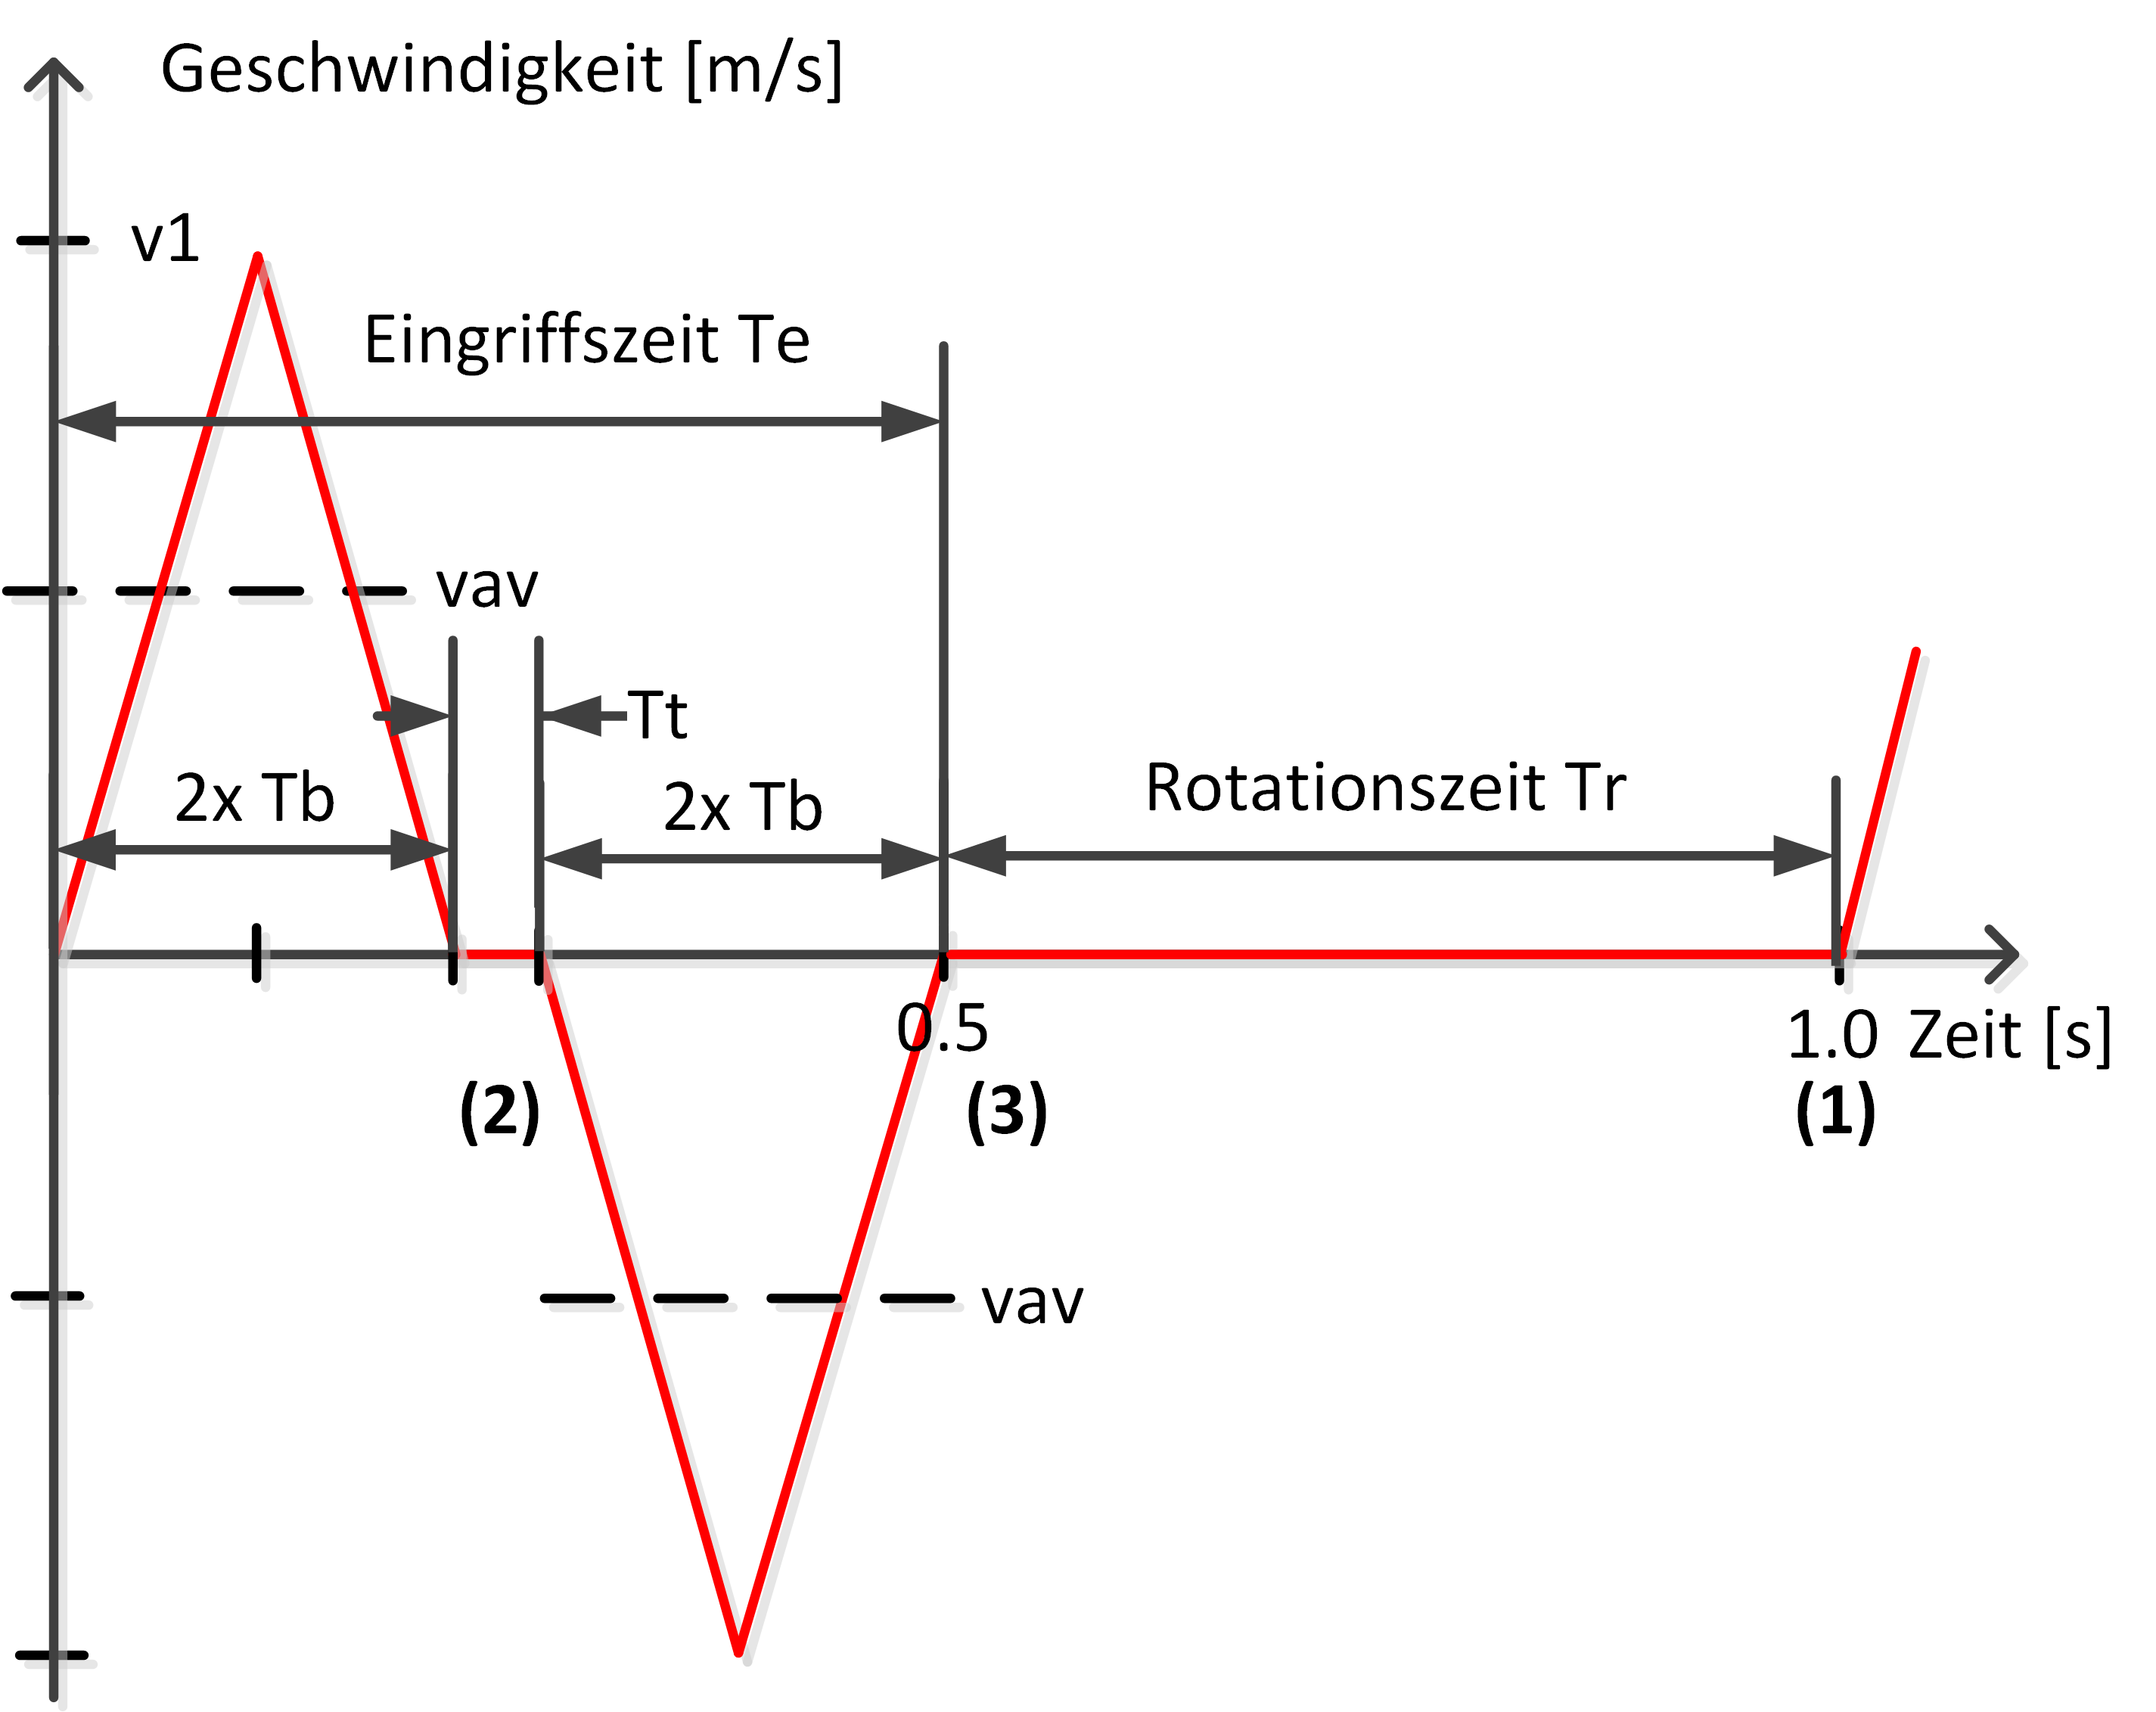
\includegraphics[width=1\textwidth]{Illustrationen/6-Umsetzung/vprofil_dorn.png}
	\caption{Geschwindigkeitsprofil des Dorns}
	\label{fig:vprofil_dorn}
\end{figure}
Orientiert an den Anforderungen aus Kapitel \ref{subsec:Translation} und der berrechneten Geschwindigkeit sind vier Steilgewindespindeln von Igus ausgewählt worden. In Rücksprache mit Mark Chalençon, Produktmanager bei igus Schweiz GmbH, wurde die Auswahl der Produkte zusätzlich verifiziert (Mail vom 18.4.17).
\begin{table}[H]
\begin{tabular}{|c|c|}
	\hline 
	Ds14x30 (Edelstahl) & Ds10x25 (Edelstahl) \\ 
	\hline 
	Ds14x30 (Aluminium) & Ds10x25 (Aluminium) \\ 
	\hline 
\end{tabular} 
\caption{Ausgewählte Steilgewindespindeln von Igus}
\label{tab:spindeln}
\end{table}
Mit diesen Angaben kann die Spindel nach Wittel, Muhs, Jannasch und Vossiek (2013) durch ein reduziertes Model dargestellt werden (analog zu Abbildung 13-5, S.448):
 	\begin{figure}[H]
 	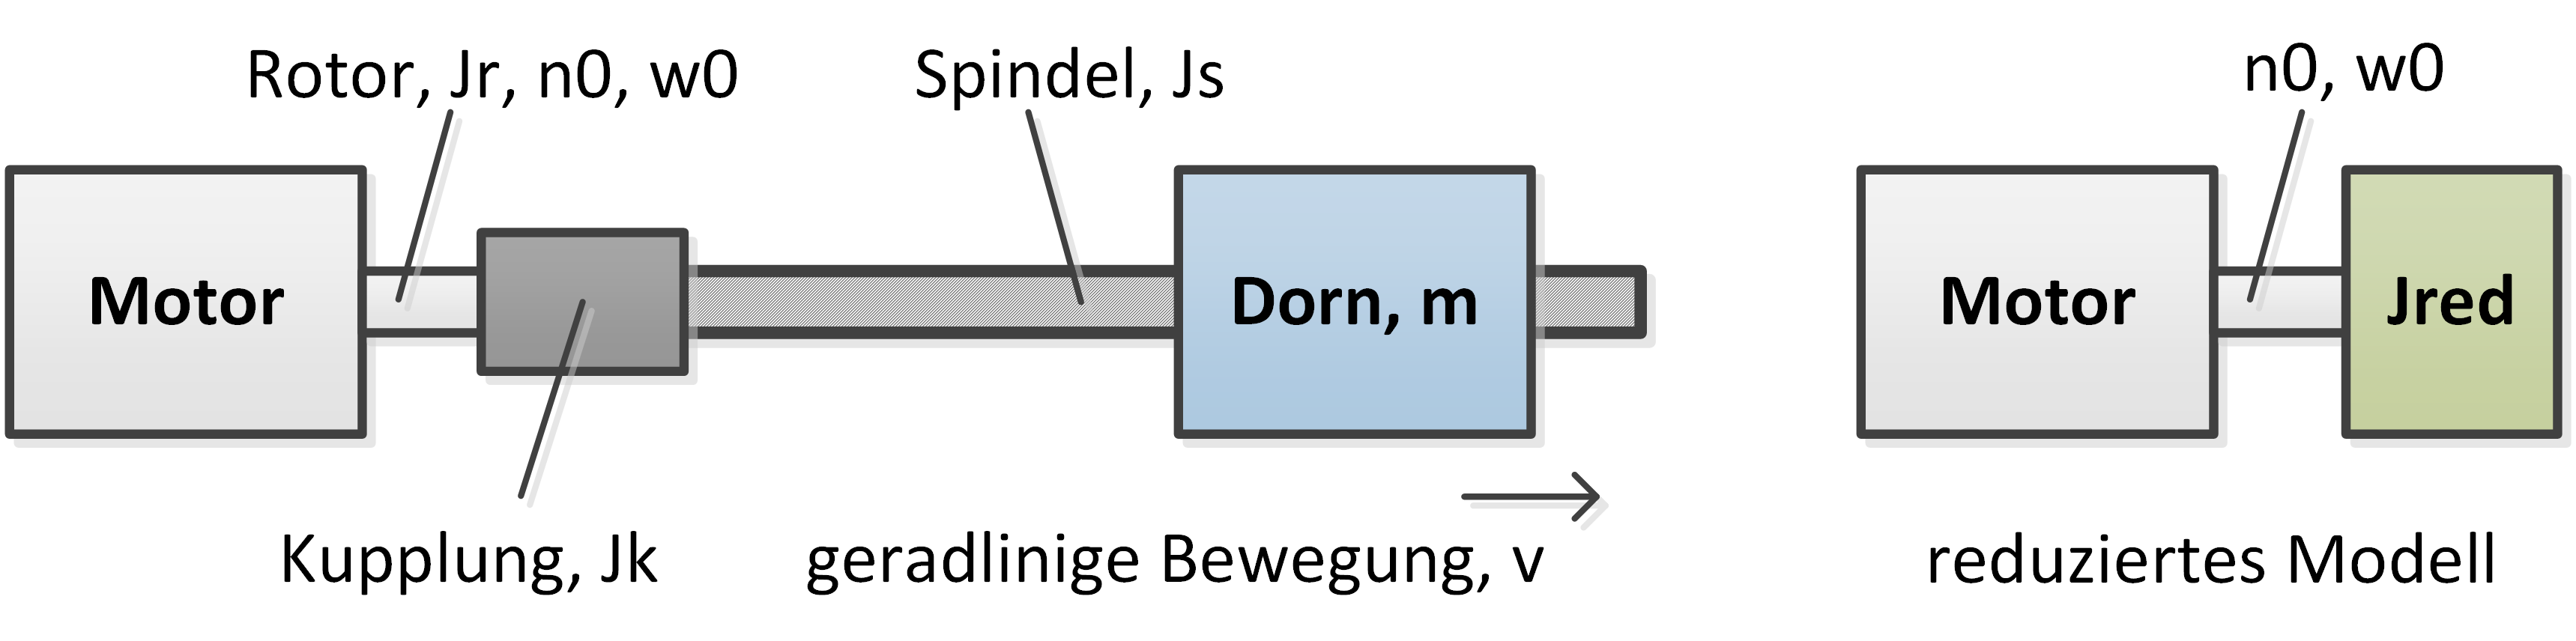
\includegraphics[width=1\textwidth]{Illustrationen/6-Umsetzung/red_modell.png}
 	\caption{Schema des Spindelantriebs sowie des reduzierten Modells}
 	\label{fig:red_modell}
	\end{figure}
wobei für das reduzierte Modell sich die reduzierte Massenträgheit Jred und das benötigte Beschleunigungsmoment Ma ergibt (Gleichung 13.3 und 13.4, S.449):
\begin{equation}
J_{red}=J_{rotor}+J_{kupplung}+J_{spindel}+m*(\frac{v_{1}}{w_{0}})^{2}
\end{equation}
\begin{equation}
M_{a}=J_{red}*\frac{w_{2}-w_{1}}{t_{b}}=J_{red}*\frac{w_{0max}}{t_{b}}
\end{equation}
Für die ausgewählten Spindeltypen ergibt dies folgende Werte:
\newline
\textbf{Tabelle der Spindeln}
\newline
\newline
Als definitive Wahl wird die Spindel Ds10x25 aus Edelstahl ausgewählt. Folgende Argumente sind relevant:
	\begin{itemize}
	\item Die Variante Ds10x25 aus Edelstahl bietet das Optimum von geringem Durchmesser und hoher Festigkeit. Das leicht höhere Beschleunigungsmoment der Ds10x25 aus Edelstahl zur Ds14x30 wird für eine höhere Festigkeit in Kauf genommen.
	
	\item \ Die geringere Steigung gibt dem Motor mehr Weg (Umdrehungen) zur Beschleunigung.
\end{itemize}